\def\mytitle{CIRCLE ASSIGNMENT}
\def\myauthor{Divya Sai}
\def\contact{nanneboinadivyasai@.com}
\def\mymodule{Future Wireless Communication (FWC)}
\documentclass[10pt, a4paper]{article}
\usepackage[a4paper,outer=1.5cm,inner=1.5cm,top=1.75cm,bottom=1.5cm]{geometry}
\twocolumn
\usepackage{graphicx}
\graphicspath{{./images/}}
\usepackage[colorlinks,linkcolor={black},citecolor={blue!80!black},urlcolor={blue!80!black}]{hyperref}
\usepackage[parfill]{parskip}
\usepackage{lmodern}
\usepackage{tikz}
 \usepackage{physics}
%\documentclass[tikz, border=2mm]{standalone}
\usepackage{karnaugh-map}
%\documentclass{article}
\usepackage{tabularx}
\usepackage{circuitikz}
\usetikzlibrary{calc}
\usepackage{amsmath}
\usepackage{amssymb}
\renewcommand*\familydefault{\sfdefault}
\usepackage{watermark}
\usepackage{lipsum}
\usepackage{xcolor}
\usepackage{listings}
\usepackage{float}
\usepackage{titlesec}
\providecommand{\mtx}[1]{\mathbf{#1}}
\titlespacing{\subsection}{1pt}{\parskip}{3pt}
\titlespacing{\subsubsection}{0pt}{\parskip}{-\parskip}
\titlespacing{\paragraph}{0pt}{\parskip}{\parskip}
\newcommand{\figuremacro}[5]{
    \begin{figure}[#1]
        \centering
        \includegraphics[width=#5\columnwidth]{#2}
        \caption[#3]{\textbf{#3}#4}
        \label{fig:#2}
    \end{figure}
}
\newcommand{\myvec}[1]{\ensuremath{\begin{pmatrix}#1\end{pmatrix}}}
\let\vec\mathbf
\lstset{
frame=single, 
breaklines=true,
columns=fullflexible
}

\title{\mytitle}
\author{\myauthor\hspace{1em}\\\contact\\FWC22094\hspace{6.5em}IITH\hspace{0.5em}\mymodule\hspace{6em}MATRICES}
\date{}
\begin{document}
 \maketitle
 \paragraph*{\large Problem Statement}
$-$ \textbf{ Let C be the circle with center at (1,1) and radius is 1.If T is the circle centered at (0,y) passing through origin and touching the circle C externally,then the radius of T is equal to:}
 
\begin{figure}[h]
\centering
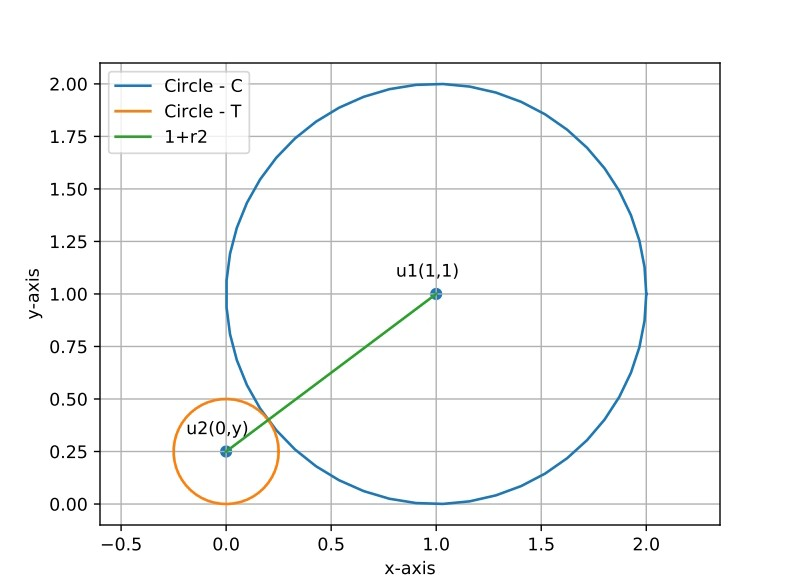
\includegraphics[width=1\columnwidth]{circle.jpeg}
\end{figure}
 \section*{Construction}
\vspace{2mm}
 The input parameters are as follows
{
\setlength\extrarowheight{4pt}
\begin{center}
 \begin{tabular}{|c|c|c|}
 \hline
 \textbf{Symbol}&\textbf{Value}&\textbf{Description}\\
 \hline
 $r_1$&$
 1$
 &radius  \\
 \hline
 $r_2$&$
 y$
 &radius\\
 \hline
 
 $u_1$&$
 \begin{pmatrix}
  1\\
  1\\
 \end{pmatrix}$
 &center\\
 \hline
 $u_2$&$
 \begin{pmatrix}
  0\\
  y\\
 \end{pmatrix}$
 &center\\
 \hline
 
 \end{tabular}
 \end{center}
}
\section*{\large solution}

\subsection*{\large step 1}
The general equation of the circle is
\begin{align}
\vec{x}^{\top}\vec{V}\vec{x}+2\vec{u}^{\top}\vec{x}+f=0
\end{align}
where V is the identity matrix
\\Let the equation of the circle C with radius $\vec{r_1}$ and center $\vec{u_1}$
\begin{align}
\vec{x}^{\top}\vec{x}+2\vec{u_1}^{\top}\vec{x}+f_1=0
\end{align}
Equation of the circle T with center $\vec{u_2}$ and radius $\vec{r_2}$
\begin{align}
\vec{x}^{\top}\vec{x}+2\vec{u_2}^{\top}\vec{x}+f_2=0
\end{align}\\
Radius of circle T is the distance between origin and center,\\
\raggedright \large 
\begin{equation}
\vec{r_2}={\vec{\|u_2-O\|}}
\end{equation}
\begin{equation}
r_2=\sqrt{{\myvec{0 && y} }{\myvec{0 \\ y}}}
\end{equation}
\begin{equation}
\boxed{r_2=y}
\end{equation}
Distance between $\vec{u_1}$ and $\vec{u_2}$:
\raggedright \large 
\begin{equation}
\vec{d}={\vec{\|u_1-u_2\|}}
\end{equation}
\begin{equation}
\vec{d}=1+r_2
\end{equation}
\begin{equation}
r_1+r_2=\vec{\|u_1 -u_2\|} 
\end{equation}
\begin{equation}
(r_1+r_2)^2=\vec{\|u_1 -u_2\|}^2 
\end{equation}
\begin{equation}
r_1^2 + r_2^2 +2 r_1 r_2=\vec{\|u_1 \|}^2 + \vec{\|u_2\|}^2 -2  u_1 ^{\top} u_2 
\end{equation}
\begin{equation}
1+r_2^2 +2 r_2= 2+r_2^2 -2{\myvec{1 && 1} }{\myvec{0 \\ r_2} }
\end{equation}
\begin{equation}
1+2 r_2=2-2 r_2
\end{equation}
\begin{equation}
4 r_2=1
\end{equation}
\begin{equation}
\boxed{$$r_2$=1/4$}
\end{equation}
\vspace{2mm} 
\vspace{5mm}
 \vspace{2mm} 
\end{document}
